\documentclass[10pt]{article}

\usepackage{mdwlist}
\usepackage[a4paper]{geometry}
\usepackage{listings}
\usepackage{graphicx}
\usepackage{float}

\title{Distributed Systems Programming - Coursework 1}
\author{Joseph Davidson \\  071729468}
\date{}

\begin{document}

  \maketitle

  \section{Introduction and Assumptions}
    This document constitutes the submission by Joseph Davidson for
    the Distributed Systems Programming coursework 1 set by Andrew Ireland.
    
    This coursework concentrates on the modelling of the absolute block
    system for railway safety. I made the following assumptions which are
    listed below:
    \begin{itemize*}
      \item The track side circuits (modelled by a channel from the signal
            to the signal box) are instantaneous because they are electric.
      \item For the purposes of the modelling, there is a continuous loop of
            trains so the system will not reach an end state.
      \item That the accuracy of the model was of a very high importance.
    \end{itemize*}
    
   
  \section{Diagrammatic Representation}
    The model I created models all of the protocols detailed in the
    specification document. To this end, it is quite a complicated model
    with much communication between processes. A diagram of the system 
    (without the monitor process) is below:
    \begin{figure}[H]
      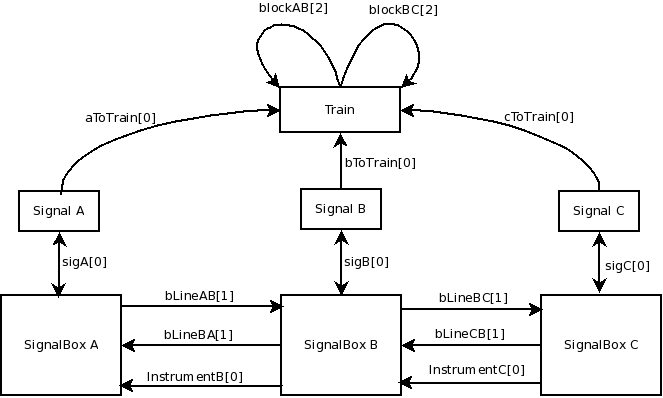
\includegraphics[scale=0.6]{diagram.png}
    \end{figure}

  \section{Verification task}
    Verification of the system using xspin is a Goddamn nightmare. Promela has
    some idiosyncrasies that result in illogical execution of statements.
    For instance, in an infinite loop, statements that block are evaluated 
    once. If they should actually block, they're silently skipped. First the
    check using the infinite train model, then I will go into details on some
    problems I have encountered using the language.  

    The infinite train forking and continuous nature of the system makes
    standard verification impossible. Checking for invalid end states cannot
    be done because the system doesn't end but the real rub is that the system
    technically doesn't repeat itself so it can't just see that it's in a loop.
    We can show that it is in a loop by considering the Train process. Every 
    time it forks, it creates a child process that does exactly the same thing
    as its parent, but has a different pid, because of this, the verifier always
    thinks that something new is happening and doesn't recognise the loop.
    
    The output of the standard vanilla check is below, it checks the assertion
    (nfull(blockAB) \&\& nfull(blockBC) only:

    \begin{verbatim}
pan: error, VECTORSZ too small, recompile pan.c with -DVECTORSZ=N with N>1024
pan:1: aborting (at depth 8952)
pan: wrote pan_in.trail

(Spin Version 5.2.5 -- 17 April 2010)
Warning: Search not completed
	+ Partial Order Reduction

Full statespace search for:
	never claim         	- (not selected)
	assertion violations	+
	cycle checks       	- (disabled by -DSAFETY)
	invalid end states	- (disabled by -E flag)

State-vector 1024 byte, depth reached 8952, errors: 1
     7380 states, stored
        0 states, matched
     7380 transitions (= stored+matched)
        0 atomic steps
hash conflicts:         0 (resolved)

Stats on memory usage (in Megabytes):
    7.291	equivalent memory usage for states (stored*(State-vector + overhead))
    4.491	actual memory usage for states (compression: 61.59%)
         	state-vector as stored = 626 byte + 12 byte overhead
    2.000	memory used for hash table (-w19)
    0.305	memory used for DFS stack (-m10000)
    6.700	total actual memory usage


pan: elapsed time 0.07 seconds
pan: rate 105428.57 states/second
pan: avg transition delay 9.4851e-06 usec
0.04user 0.02system 0:00.08elapsed 86%CPU (0avgtext+0avgdata 0maxresident)k
0inputs+0outputs (0major+1863minor)pagefaults 0swaps


    \end{verbatim}

    \subsection{Promela Issues}
      I wanted to evaluate the system using only a few trains instead of an
      infinite number. I elected to modify the Train process to accommodate
      a variable that decided whether to fork the Train process or not. This
      involved passing a byte from parent process to child that, if it was
      greater than 0, was decremented and passed to the child. The child that
      had a 0 passed to it would not fork and the processes would all
      terminate.

      I wrote a simple if statement that compared a value \textit{next} and
      forked if it succeeded and just continued if it didn't:

      \begin{verbatim}
        if:: (next>0) -> run Train(aSig, bSig, cSig, sectAB, sectBC, next-1);
          :: else ->;  
        fi;  
      \end{verbatim}
   
      This code results in an assertion violation. For some unknown reason,
      this statement blocks in the second last train that is run and I've
      tried every variant and deviant of that code to try and make the
      second last run possible. 
      I honestly have no idea whatsoever as to why this happens. Given an
      infinite number of train, the system works perfectly until it runs
      out of space. But given a finite number, the program would die at the
      second last train.

      I finally fixed the problem by moving the fork to the very end of the
      Train process. I feel that this is a bit cheating as moving the fork to
      the end ensures that the previous train is totally off the track before
      a new comes on. Regardless, the output is below for 7 trains:
      \begin{verbatim}
Spin Version 5.2.5 -- 17 April 2010)
	+ Partial Order Reduction

Full statespace search for:
	never claim         	- (not selected)
	assertion violations	+
	cycle checks       	- (disabled by -DSAFETY)
	invalid end states	- (disabled by -E flag)

State-vector 208 byte, depth reached 700, errors: 0
     5597 states, stored
     4686 states, matched
    10283 transitions (= stored+matched)
        0 atomic steps
hash conflicts:        28 (resolved)

Stats on memory usage (in Megabytes):
    1.174	equivalent memory usage for states (stored*(State-vector + overhead))
    1.254	actual memory usage for states (unsuccessful compression: 106.81%)
         	state-vector as stored = 223 byte + 12 byte overhead
    2.000	memory used for hash table (-w19)
    0.305	memory used for DFS stack (-m10000)
    3.477	total actual memory usage


pan: elapsed time 0.03 seconds
pan: rate 186566.67 states/second
pan: avg transition delay 2.9174e-06 usec
0.03user 0.00system 0:00.03elapsed 91%CPU (0avgtext+0avgdata 0maxresident)k
0inputs+0outputs (0major+1040minor)pagefaults 0swaps
      \end{verbatim} 

    \subsection{Progress Cycles}
      Because the system basically runs in an infinite loop, progress cycle
      checking was used to make sure that the program looped with progress.
      Progress labels were placed in the processes and the verifier was run.
      Here are the results for 7 trains:
      \begin{verbatim}
Spin Version 5.2.5 -- 17 April 2010)
	+ Partial Order Reduction

Full statespace search for:
	never claim         	+
	assertion violations	+ (if within scope of claim)
	non-progress cycles 	+ (fairness disabled)
	invalid end states	- (disabled by never claim)

State-vector 248 byte, depth reached 1971, errors: 0
     9690 states, stored
     9363 states, matched
    19053 transitions (= stored+matched)
        0 atomic steps
hash conflicts:        81 (resolved)

Stats on memory usage (in Megabytes):
    2.440	equivalent memory usage for states (stored*(State-vector + overhead))
    1.645	actual memory usage for states (compression: 67.42%)
         	state-vector as stored = 162 byte + 16 byte overhead
    2.000	memory used for hash table (-w19)
    0.305	memory used for DFS stack (-m10000)
    3.868	total actual memory usage


pan: elapsed time 0.09 seconds
pan: rate 107666.67 states/second
pan: avg transition delay 4.7237e-06 usec
0.08user 0.00system 0:00.09elapsed 93%CPU (0avgtext+0avgdata 0maxresident)k
0inputs+0outputs (0major+1136minor)pagefaults 0swaps
      \end{verbatim}  

    \subsection{LTL Properties}
      Using the never claim []!(p$\mid\mid$q) where p is defined as \emph{
      full(blockAB)} and q is \emph{full(blockBC)}. This never claim is
      asserted to be an invariant throughout the program.
      (if I have [](p\&\&q) p = \emph{nfull(blockAB)} and q =
      \emph{nfull(blockBC)} with this being desired behaviour, I get an
      error).
      Here are the results for a LTL verification with 7 trains:
      \begin{verbatim}
Warning: for p.o. reduction to be valid the never claim must be stutter-invariant
(never claims generated from LTL formulae are stutter-invariant)
depth 0: Claim reached state 5 (line 353)

(Spin Version 5.2.5 -- 17 April 2010)
	+ Partial Order Reduction

Full statespace search for:
	never claim         	+
	assertion violations	+ (if within scope of claim)
	acceptance   cycles 	+ (fairness disabled)
	invalid end states	- (disabled by never claim)

State-vector 244 byte, depth reached 1969, errors: 0
     9310 states, stored
     4040 states, matched
    13350 transitions (= stored+matched)
        0 atomic steps
hash conflicts:        44 (resolved)

Stats on memory usage (in Megabytes):
    2.308	equivalent memory usage for states (stored*(State-vector + overhead))
    1.547	actual memory usage for states (compression: 67.00%)
         	state-vector as stored = 158 byte + 16 byte overhead
    2.000	memory used for hash table (-w19)
    0.305	memory used for DFS stack (-m10000)
    3.770	total actual memory usage


pan: elapsed time 0.05 seconds
pan: rate    186200 states/second
pan: avg transition delay 3.7453e-06 usec
0.04user 0.00system 0:00.04elapsed 91%CPU (0avgtext+0avgdata 0maxresident)k
0inputs+0outputs (0major+1120minor)pagefaults 0swaps
      \end{verbatim}
      
      The first message about stutter invariance is totally invalid because
      the prewritten formulae actually throws errors by the never claim
      generator because of the whitespace in the formulae.   

  \section{Log}
    Promela itself is a very persnickety language. For instance, a blocking
    if statement inside an infinite loop will proceed as if it wasn't blocked
    at all (i.e. the block has no effect). For this reason, goto statements
    had to be utilised so that the program could execute correctly.

   \subsection{Protocols, Processes and Channels}
    I made the choice to model the protocols in detail from the beginning
    of the task. I chose to do this because the ABS protocol in itself, is
    correct. So closely modelling the protocol will reduce mistakes in my
    model -- any mistake that I do make will relate to the choices I made,
    not my implementation of the protocols.
  
    I first used infinite loops for the processes -- each process just running
    in a DO loop constantly -- but I encountered the continuation error
    detailed above when I used IF statements to block execution. 
    For this reason, I discarded the loops and implemented GOTOs instead.
    The process would just jump back to the start of its execution when it was
    finished.

    I used a lot of channels in the creation of the system.
    This was to simulate the ABS as closely as possible, there is up and down
    bell lines for each pair of signalboxes, control lines and channels to
    simulate communication between the signals and the trains.

    The channels between signals and the signalboxes/train are synchronised
    channels. The rationale behind this is that the signal transmits its go/stop
    signal to the train visually -- at the speed of light and that there is
    no reply necessary from the train. Similarly with the signals track side
    circuits to the signalbox, no reply is necessary from the signalbox, it is
    just an information signal.    

   \subsection{Train Process}
    I decided to model the train as a process in itself. This was to further
    enhance the realism of the model with the realisation that the train itself
    is an integral part of the ABS that has to obey the rules set out for it.

    The only processes that access the block section channels are the train and
    monitor processes. The monitor obviously checks that the block section
    channels only have 1 train in them at a time and the train process adds and
    removes itself from the channel, depending on where it is.  

    To simulate infinite trains, the train process actually forks itself. It
    does this as soon as it enters block section AB so that another is queued
    ready to go in.
   
    \subsection{Verification}
    Verifying the system was nigh impossible (see above). Because of the infinite
    Train forking, testing for non-progress cycles was required. This was achieved
    by placing progress labels in each process and using the verifier to see if there
    were non-progress cycles in the code. This was actually relatively painless
    compared to the other verification that was used.

    Spin doesn't like LTL formulae with whitespace, this is unusual seeing as all
    the example formulae have whitespace in them and, therefore don't generate
    never claims. In addition to this, choosing whether the never claim is
    desired or error behaviour determines which commands can be used to define
    the variables of the never claim. For instance, given a formula [](p\&\&q)
    with p = \emph{nfull(blockAB)} and q = \emph{nfull(blockBC)}, if the property
    is to hold true for all executions (desired behaviour), a syntax error is
    thrown. Similarly if we say that the property holds for no executions
    (error behaviour) then the verification proceeds just fine.
   
    I really just don't understand how it manages this, maybe I'm not thinking
    through correctly\ldots Regardless, the verification was done by
    implementing workarounds and assertion, progress and state invariants were
    verified.         
 
    \subsection{Conclusion}
      In conclusion, if I were to model something else, I would probably look into
      alternatives to Promela. Its seemingly unexplainable idiosyncrasies, unhelpful
      error slicing/messages and strange rules for verification really ring
      alarm bells for me. Maybe I just don't know how to use it correctly and
      all its strange behaviour is just a result of me badly programming in it,
      but I really don't like it. I'd prefer to use something different for
      model checking in future.
       
  \section{Promela Source}
   \lstinputlisting[language=Promela]{Coursework.promela}

\end{document}
